% Requirements

Users will start their design process in the Requirements package. The Requirements Organization diagram is shown in Figure \ref{fig:Requirements Organization}, which links to each applicable diagram and provides basic instructions to help users navigate. While the Requirements process is not a linear process to be accomplished at one time, it is structured in the order in which users will likely need the included diagrams.

\begin{figure}[H]
    \centering
    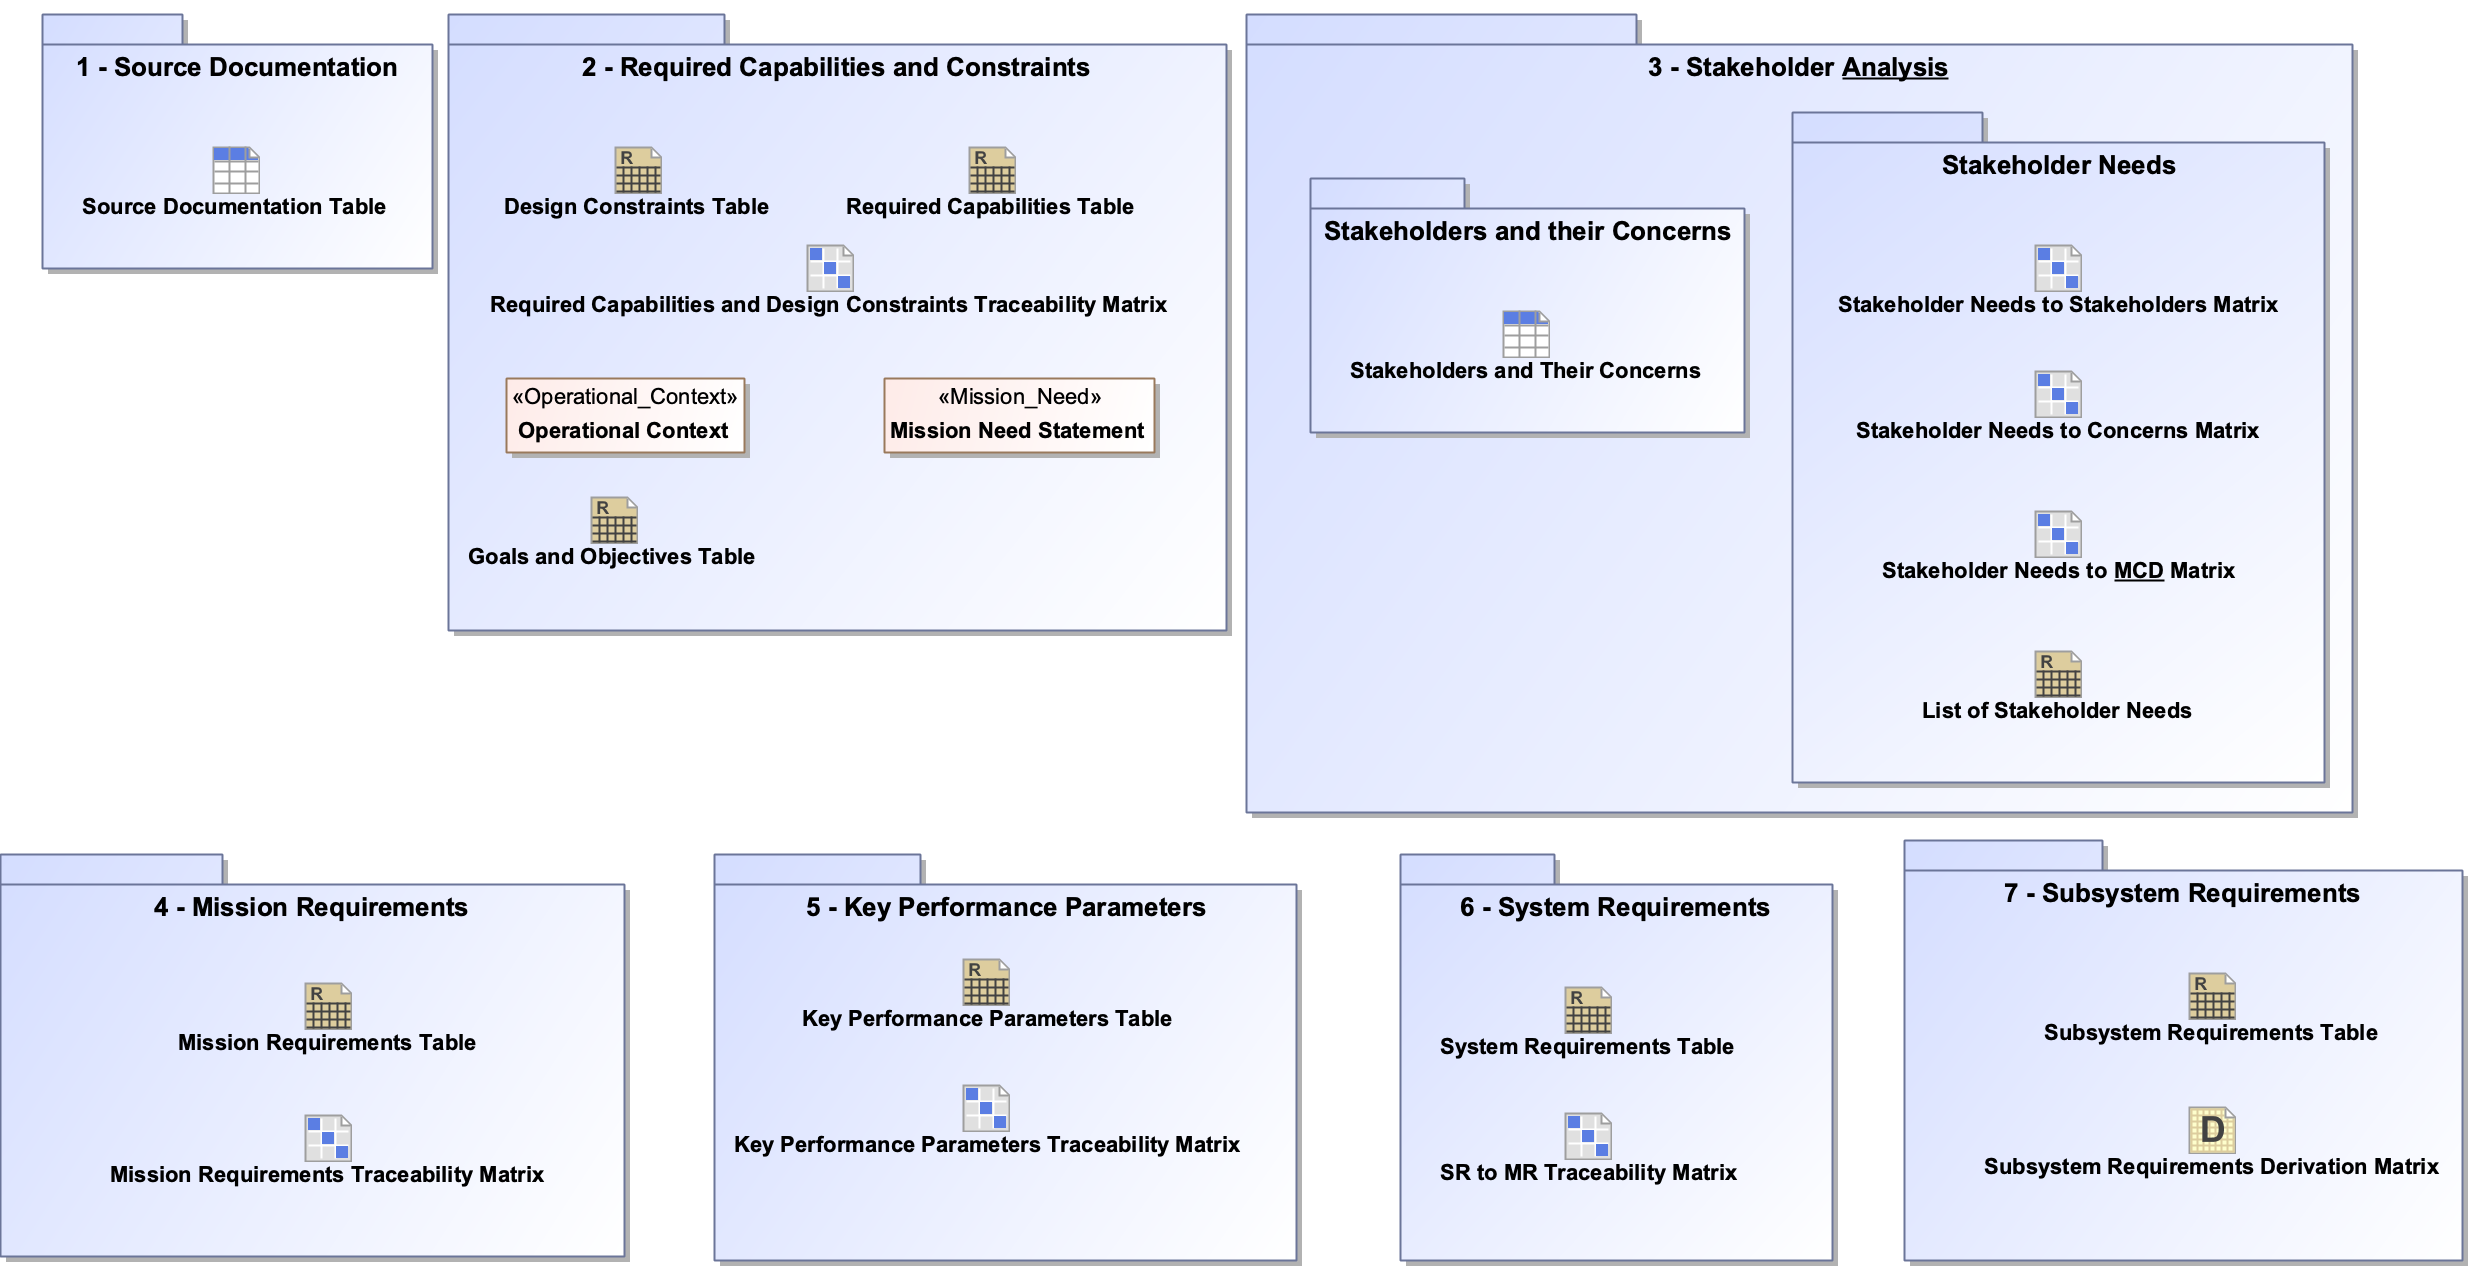
\includegraphics[scale=.5, angle=90]{Thesis/Analysis_and_Results/Analysis and Results Figures/Requirements Organization.png}
    \caption{Requirements Organization}
    \label{fig:Requirements Organization}
\end{figure}

The Requirements section begins with users creating blocks for their source material. This Source Documentation diagram will continue to grow over the course of the design sequence, but some common CubeSat references are included and attached. By attaching source material to blocks, as shown in Figure \ref{fig:Source Documentation}, requirements can be properly traced to the exact source document version. Furthermore, it makes it much easier for users to quickly see the source documentation, instead of needing to search the internet based off the source name. 

\begin{figure}[H]
    \centering
    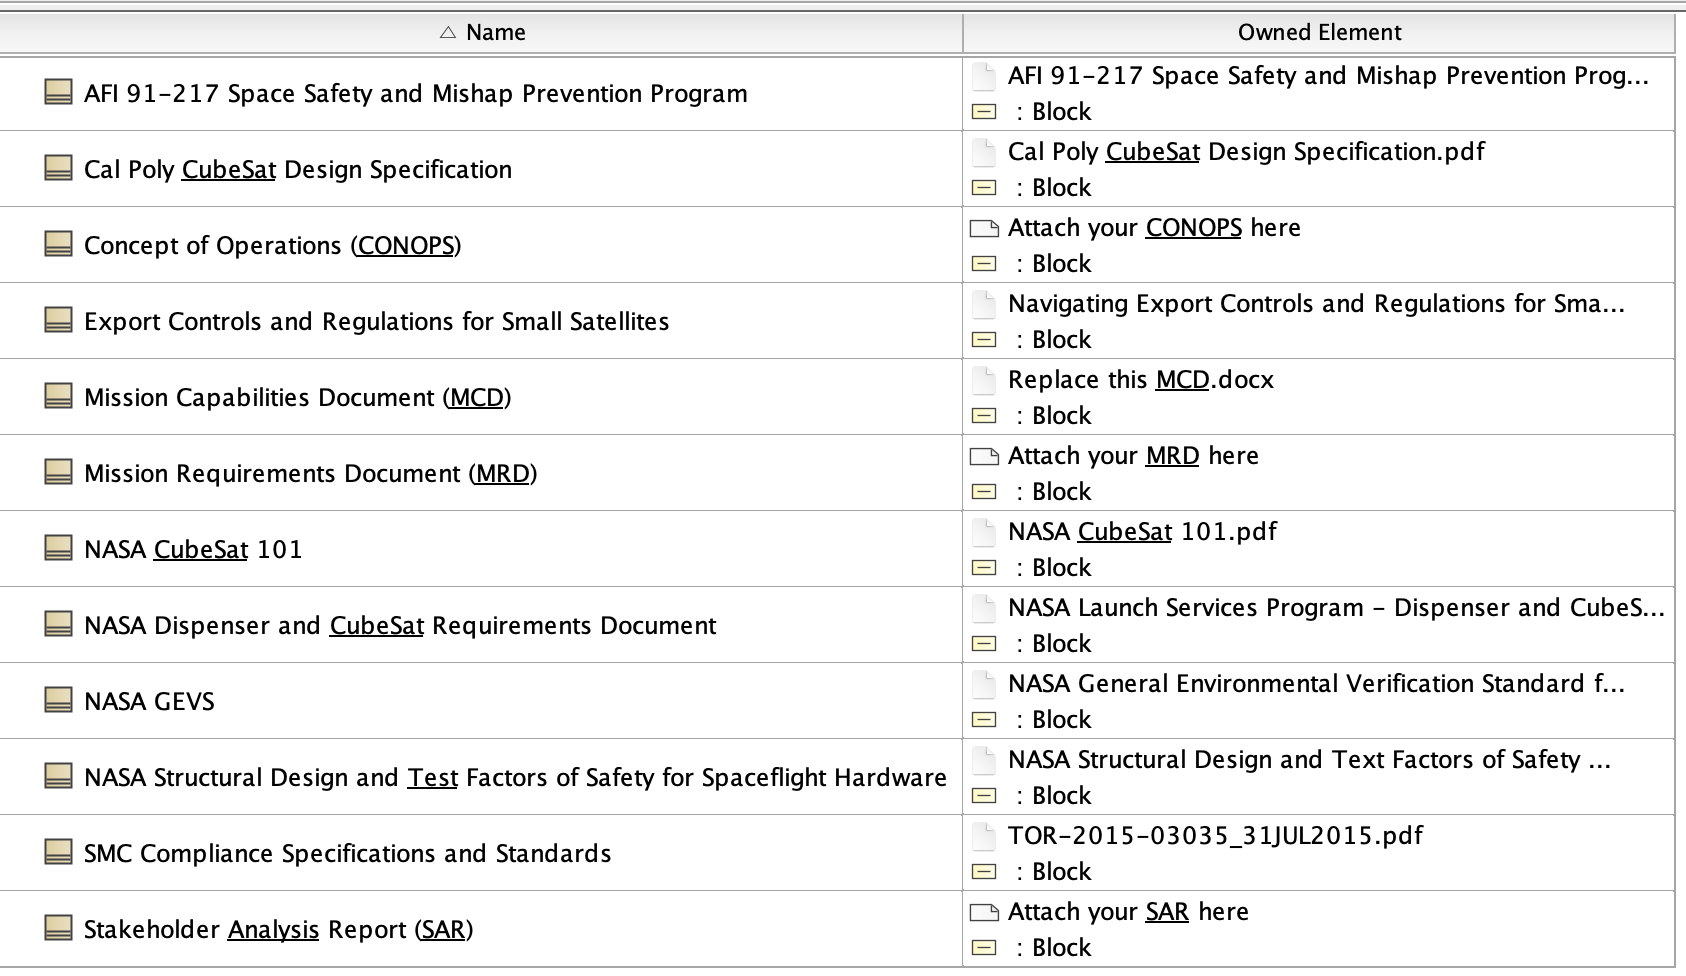
\includegraphics[width=\textwidth]{Thesis/Analysis_and_Results/Analysis and Results Figures/Source Documentation.png}
    \caption{Source Documentation}
    \label{fig:Source Documentation}
\end{figure}

The Reference Architecture assumes that design teams were provided with an MCD. Given that, users should parse the contents of the MCD into blocks that can be used within the model. Instructions are provided in the diagrams for how to accomplish this, but the goal is to have a set of Design Constraints and Required Capabilities, an Operational Context statement, a Mission Need statement, and a matrix that traces these new blocks to the MCD. If any changes occur after the original MCD was parsed, users can  generate a new MCD based off these tables using the Document Generator tool. Note also that the tables provided include an ID naming convention that will be continued when users add additional entries into the respective tables. Additionally, each table is populated with blocks that contain the correct modeling "stereotype" so that tables can properly and automatically populate. Figure \ref{fig:Design Constraints} shows an example of a Design Constraints table for one class project, and that pattern repeats for the Required Capabilities table. The tables as provided only include sample names, as these will need to be replaced as soon as an MCD is provided.

\begin{figure}[H]
    \centering
    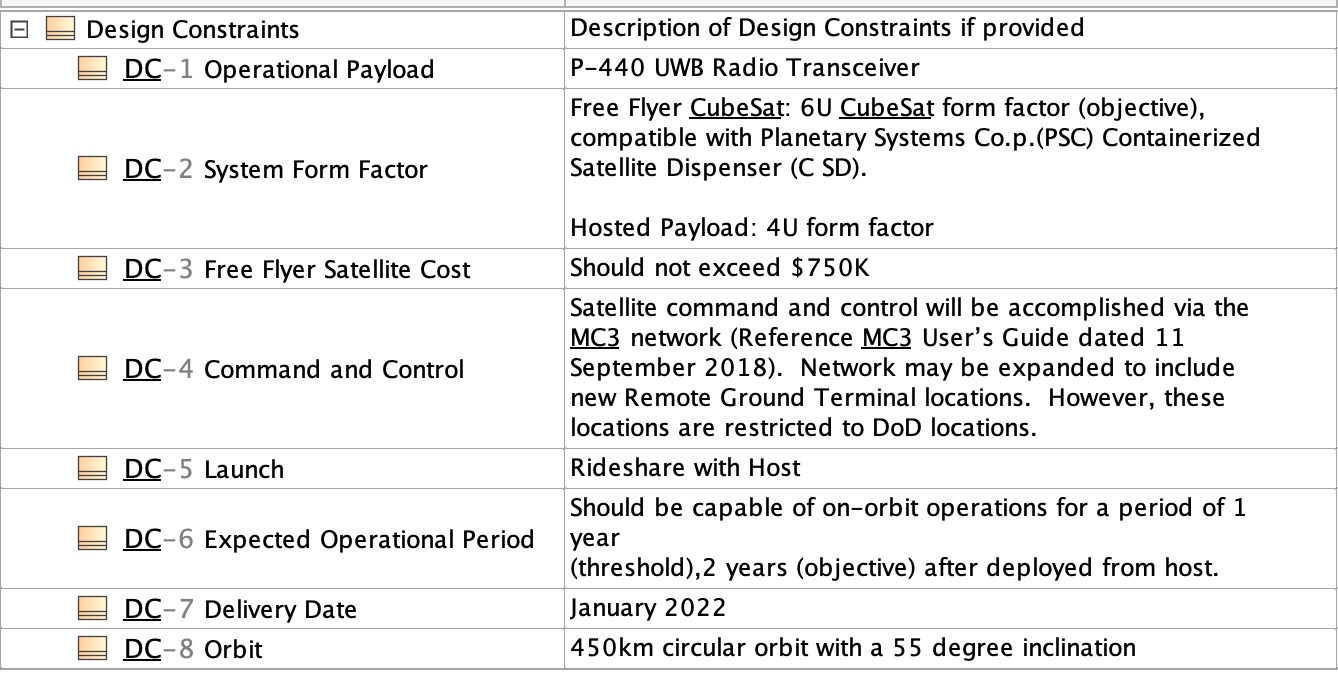
\includegraphics[width=\textwidth]{Thesis/Analysis_and_Results/Analysis and Results Figures/Design Constraints.png}
    \caption{Design Constraints}
    \label{fig:Design Constraints}
\end{figure}

The next major step is to perform a Stakeholder Analysis as a team. Figure \ref{fig:Stakeholder Analysis} shows the structure of the Stakeholder Analysis package, with a package for Stakeholder Concerns and another for Stakeholder Needs. Design teams will first brainstorm a list of Stakeholders and document whatever concerns they may have in the form of "comments" in Cameo. Some generic Stakeholders are provided as well as generic "concerns" that users should edit and add to for their unique program. The issue with these Stakeholder Concern "comments" is that requirements cannot be traced directly to them. To address this limitation, Stakeholder Needs are then created as blocks that represent those previously created concerns. Several concerns may address the same topic, so one Stakeholder Need block can be created that maps to each relevant concern. Figure \ref{fig:Stakeholder Matrix} shows a portion of the matrix that will automatically change after the previous steps. By mapping the new Need blocks to the Concern comments and to their applicable stakeholder, the user can see where each Stakeholder Need comes from. Once the team has a complete list of Stakeholder Needs with traceability back to their concerns, the Stakeholder Analysis Report can be generated. The Document Generator process will be detailed later in this chapter. 

\begin{figure}[H]
    \centering
    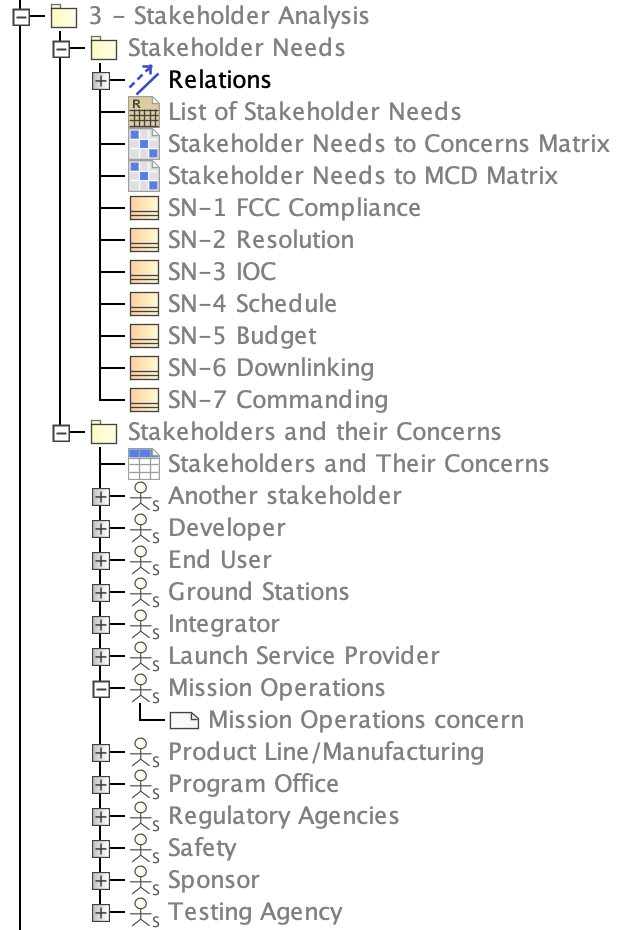
\includegraphics[width=3 in]{Thesis/Analysis_and_Results/Analysis and Results Figures/Stakeholder Containment Tree.png}
    \caption{Stakeholder Analysis}
    \label{fig:Stakeholder Analysis}
\end{figure}

\begin{figure}[H]
    \centering
    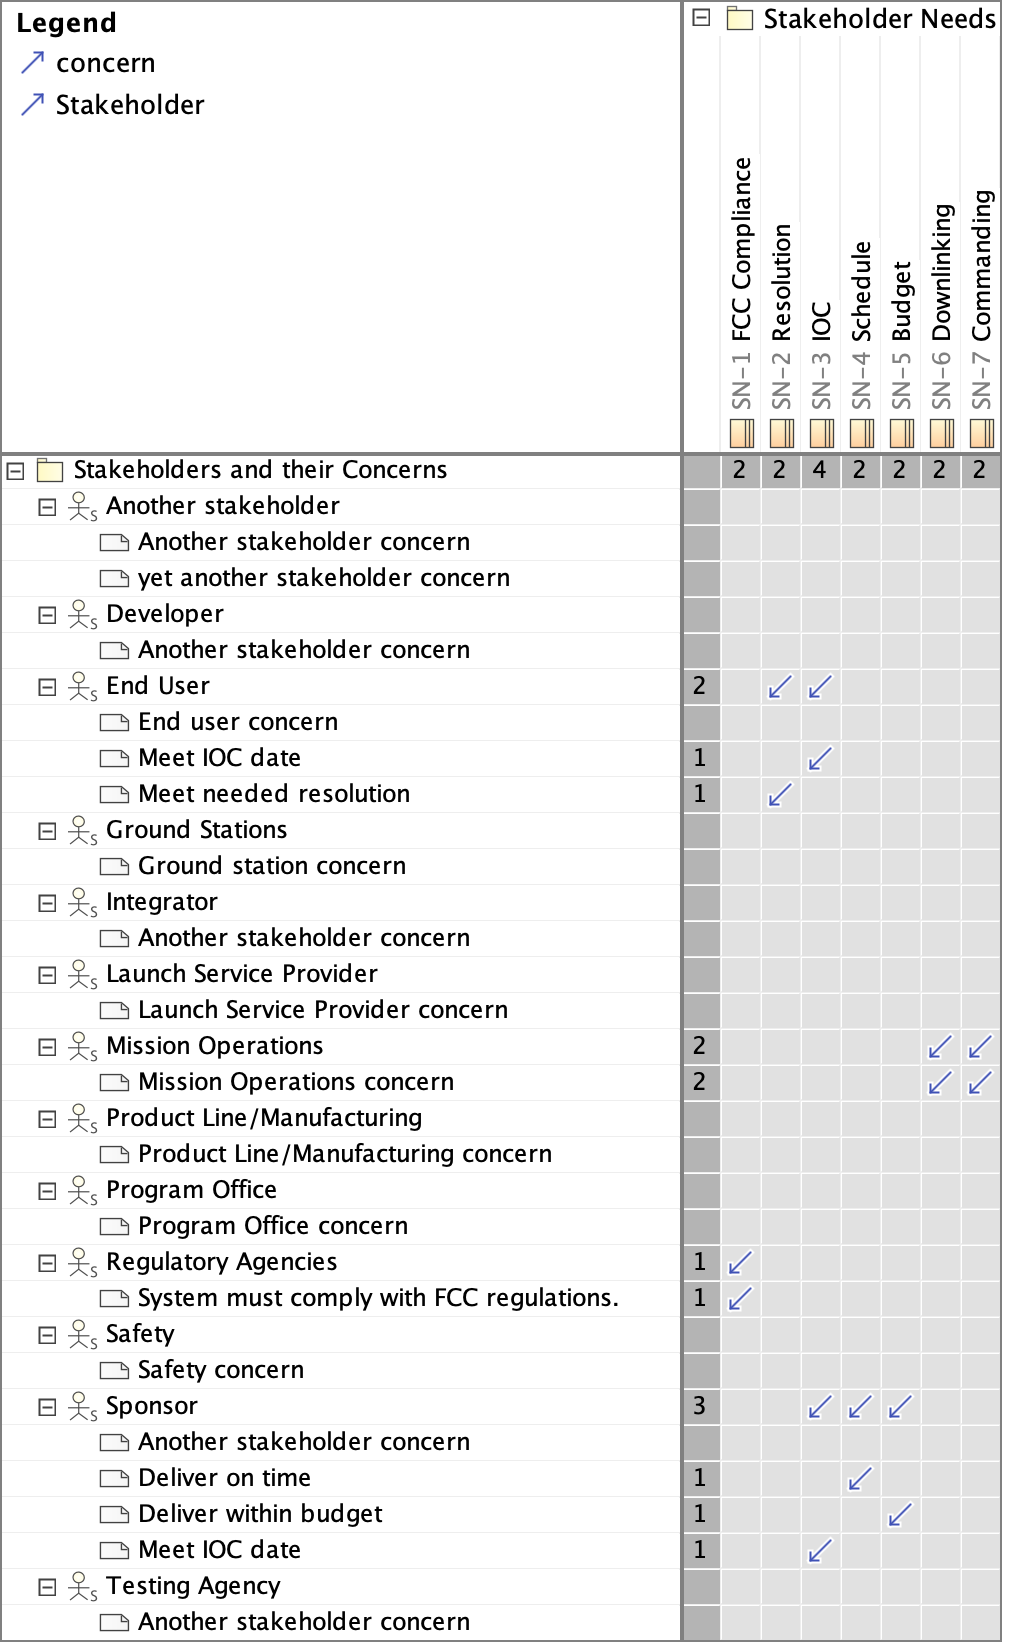
\includegraphics[width=4 in]{Thesis/Analysis_and_Results/Analysis and Results Figures/Stakeholder Matrix.png}
    \caption{Stakeholder Matrix}
    \label{fig:Stakeholder Matrix}
\end{figure}

The remaining sections within the Requirements package will be completed later in the design sequence. It is structured using a tiered Requirements convention, where teams start by generating a list of Mission Requirements, then a list of System or Space Vehicle Requirements, and finally a list of Subsystem Requirements for each subsystem. Each tier is organized in a similar fashion, but with different stereotypes and some different data fields. Additionally, template requirements for each tier have been provided, as well as some example entries in other data fields to show as examples, as shown in Figure \ref{fig:Mission Requirements}. Each tier of requirements also comes with a traceability matrix for users to trace or derive that tier from. Note that the Subsystem Requirements table, shown in Figure \ref{fig:Subsystem Requirements}, is further broken out into subsystem categories, with template requirements for each to get teams started on the brainstorming process. 

\begin{figure}[H]
    \centering
    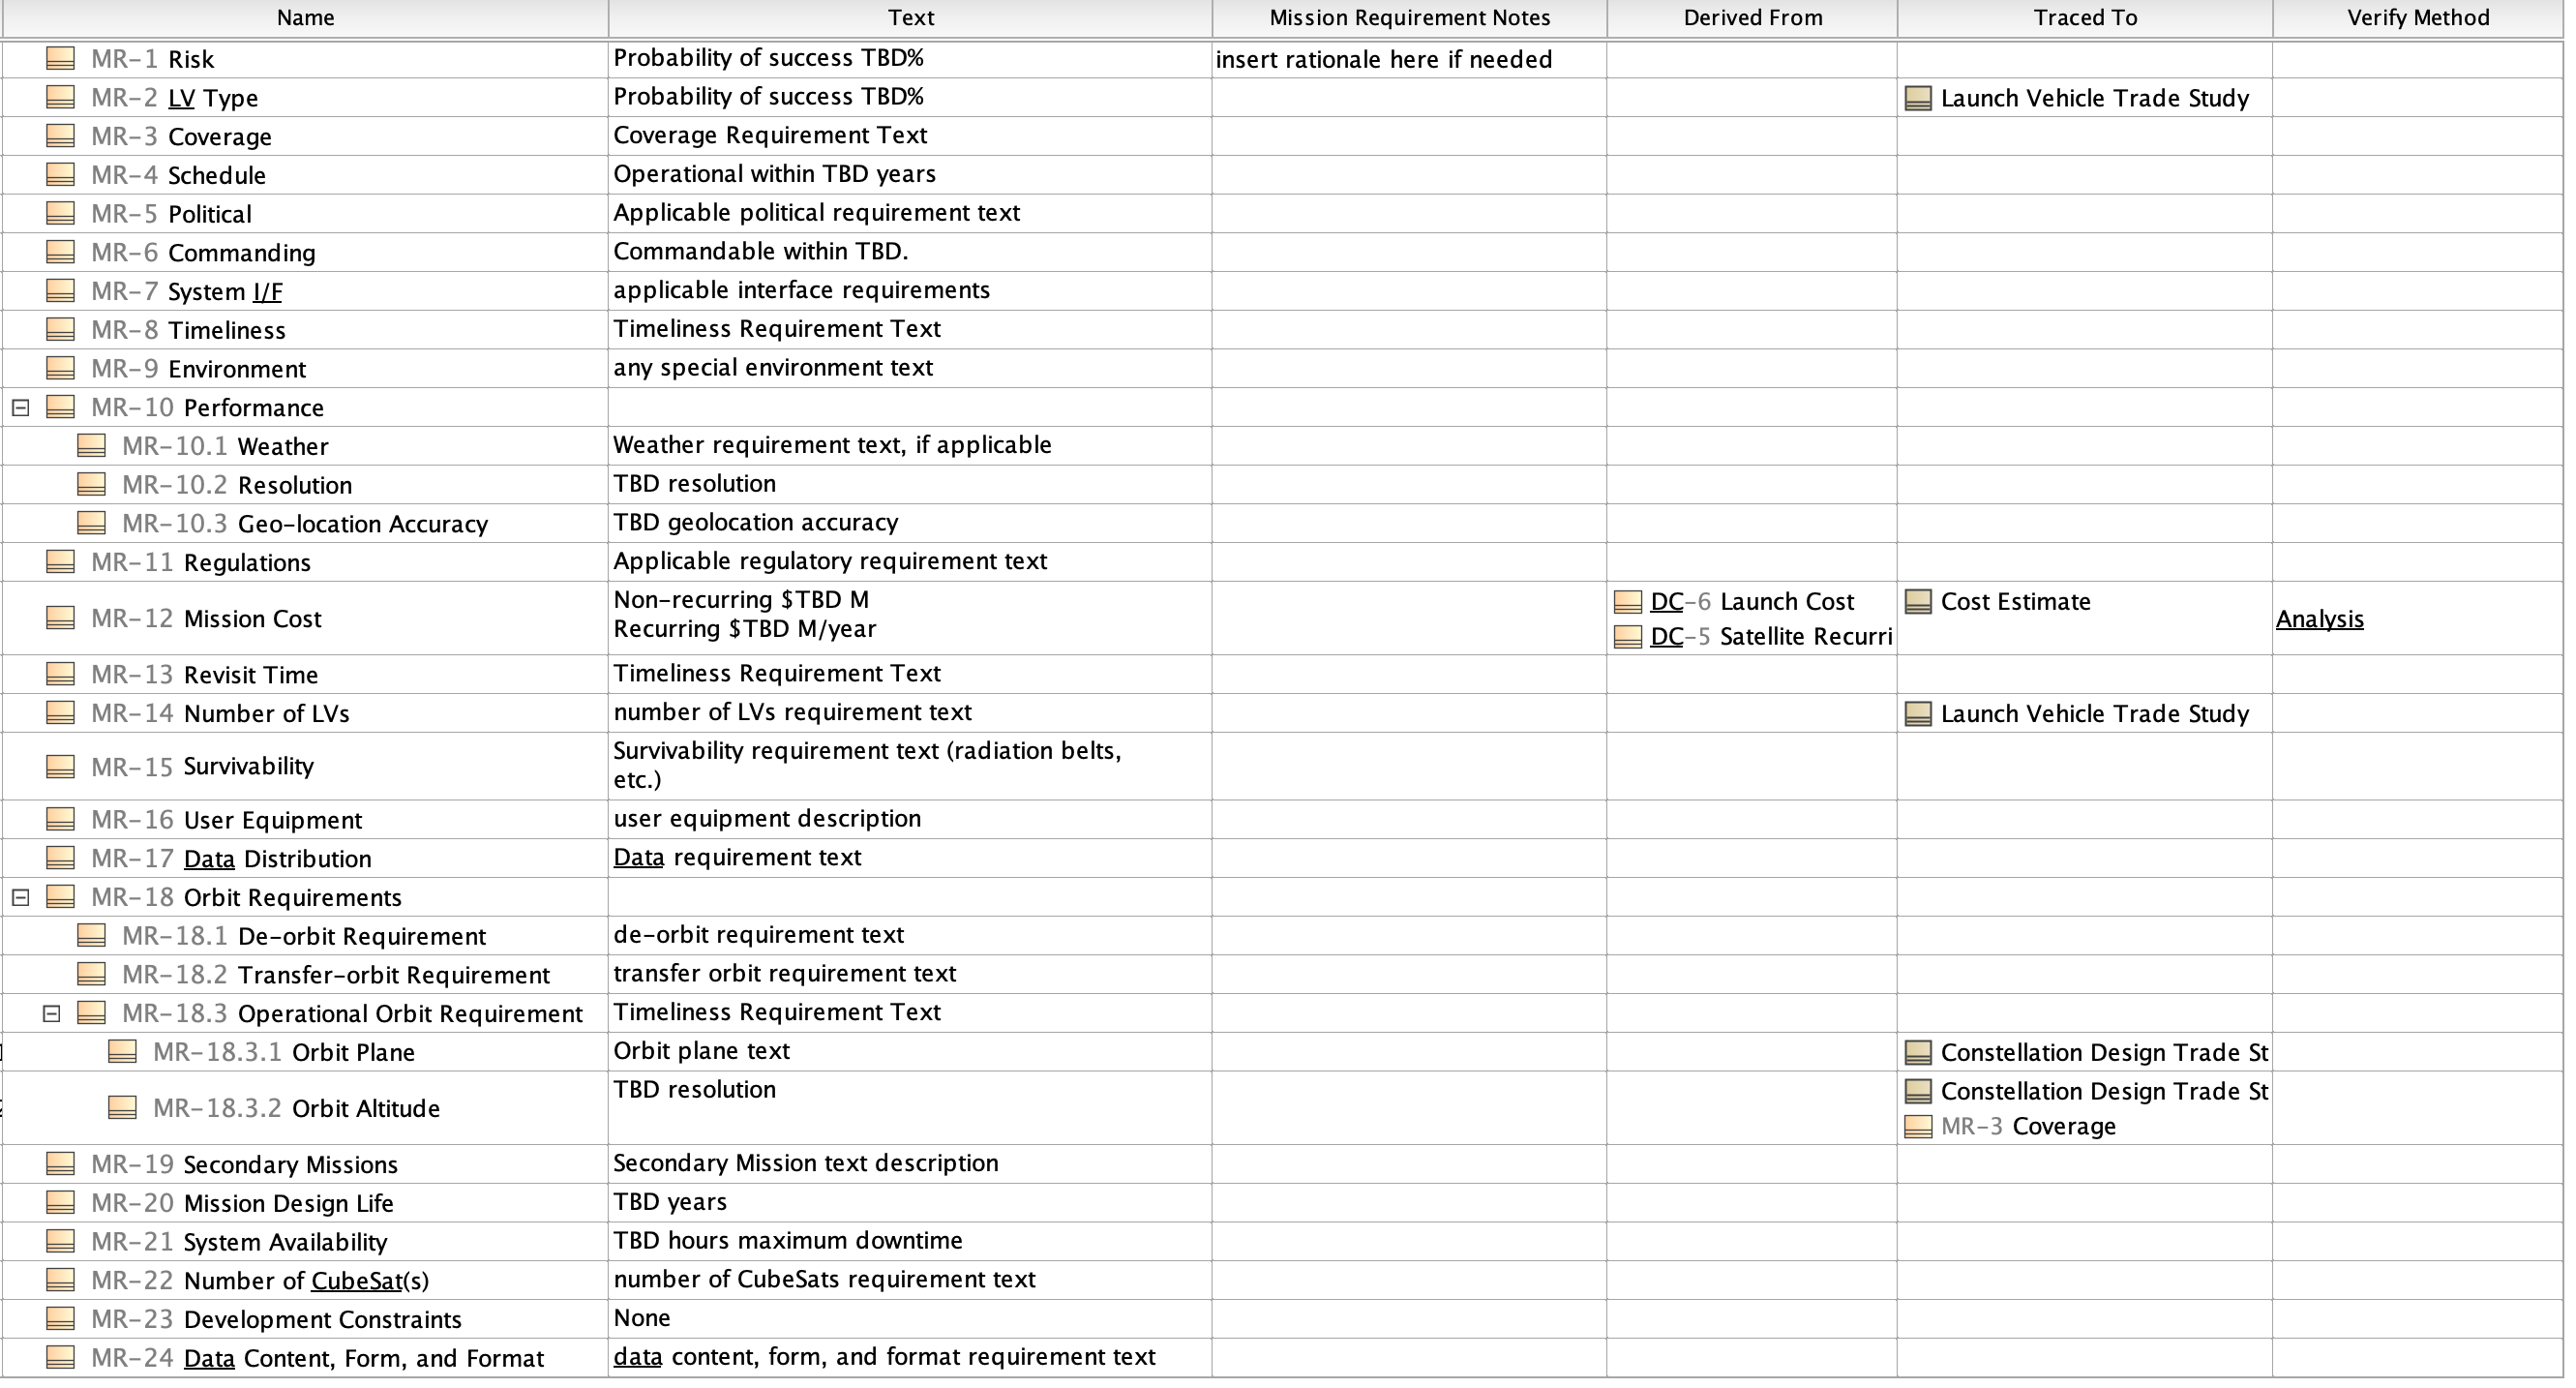
\includegraphics[width=\textwidth]{Thesis/Analysis_and_Results/Analysis and Results Figures/Mission Requirements.png}
    \caption{Mission Requirements}
    \label{fig:Mission Requirements}
\end{figure}

\begin{figure}[H]
    \centering
    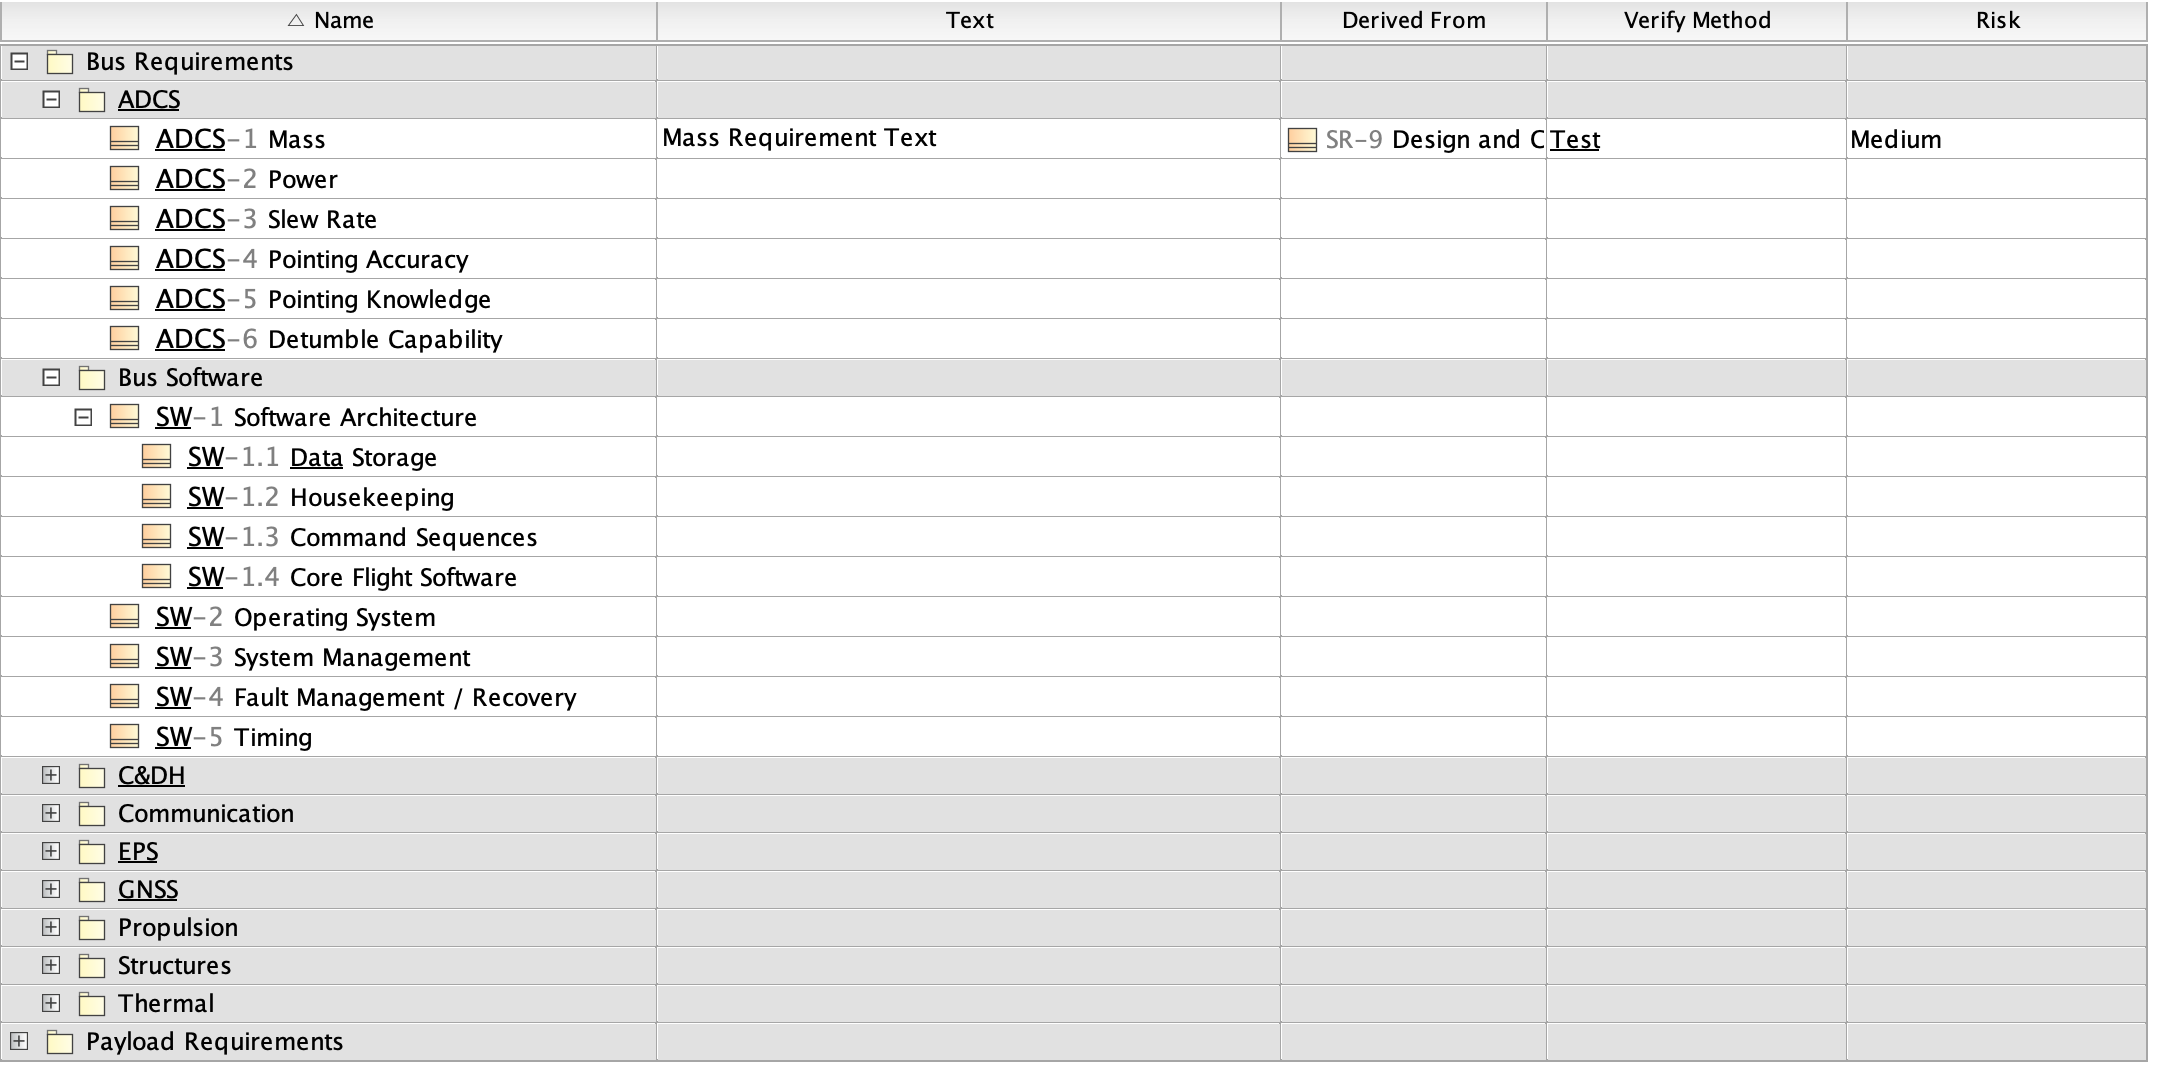
\includegraphics[width=\textwidth]{Thesis/Analysis_and_Results/Analysis and Results Figures/Subsystem Requirements.png}
    \caption{Subsystem Requirements}
    \label{fig:Subsystem Requirements}
\end{figure}